\documentclass{beamer}
\usepackage[utf8]{inputenc}

\usetheme{Madrid}
\usecolortheme{default}
\usepackage{amsmath,amssymb,amsfonts,amsthm}
\usepackage{txfonts}
\usepackage{tkz-euclide}
\usepackage{listings}
\usepackage{adjustbox}
\usepackage{array}
\usepackage{tabularx}
\usepackage{gvv}
\usepackage{lmodern}
\usepackage{circuitikz}
\usepackage{tikz}
\usepackage{graphicx}

\setbeamertemplate{page number in head/foot}[totalframenumber]

\usepackage{tcolorbox}
\tcbuselibrary{minted,breakable,xparse,skins}



\definecolor{bg}{gray}{0.95}
\DeclareTCBListing{mintedbox}{O{}m!O{}}{%
	breakable=true,
	listing engine=minted,
	listing only,
	minted language=#2,
	minted style=default,
	minted options={%
		linenos,
		gobble=0,
		breaklines=true,
		breakafter=,,
		fontsize=\small,
		numbersep=8pt,
		#1},
	boxsep=0pt,
	left skip=0pt,
	right skip=0pt,
	left=25pt,
	right=0pt,
	top=3pt,
	bottom=3pt,
	arc=5pt,
	leftrule=0pt,
	rightrule=0pt,
	bottomrule=2pt,
	toprule=2pt,
	colback=bg,
	colframe=orange!70,
	enhanced,
	overlay={%
		\begin{tcbclipinterior}
			\fill[orange!20!white] (frame.south west) rectangle ([xshift=20pt]frame.north west);
	\end{tcbclipinterior}},
	#3,
}
\lstset{
	language=C,
	basicstyle=\ttfamily\small,
	keywordstyle=\color{blue},
	stringstyle=\color{orange},
	commentstyle=\color{green!60!black},
	numbers=left,
	numberstyle=\tiny\color{gray},
	breaklines=true,
	showstringspaces=false,
}
%------------------------------------------------------------
%This block of code defines the information to appear in the
%Title page
\title %optional
{4.11.24}
%\subtitle{A short story}

\author % (optional)
{RAVULA SHASHANK REDDY - EE25BTECH11047}

 \begin{document}
	
	
	\frame{\titlepage}
	\begin{frame}{Question}
Find the equation of the plane through the line of intersection of
\begin{align*}
\vec{r}^T (\vec{i} + 3\vec{j}) + 6 = 0,
\vec{r}^T (3\vec{i} - \vec{j} - 4\vec{k}) = 0
\end{align*}
which is at unit distance from origin.\\

\end{frame}
\begin{frame}{Equation}
Family of Planes
\begin{align*}
    \vec{n}_1^T\vec{x} - c_1 +\lambda(\vec{n}_2^T\vec{x} - c_2)=0
\end{align*}
    
\end{frame}
\begin{frame}{Solution:}
Given:
\begin{align}
\pi_1 &: 
 \vec{n}_1=\myvec{1\\3\\0}, \ c_1=-6, \\[1ex]
\pi_2 &: \vec{n}_2=\myvec{3\\-1\\-4}, \ c_2=0.
\end{align}

Family of planes:
\begin{align}
(\vec{n}_1+\lambda\vec{n}_2)^T\vec{x}&=c_1+\lambda c_2\\
\vec{n}^T\vec{x}  &= c
\end{align}

Distance condition:
\begin{align}
d&=\frac{|\vec{n}^T\vec{x}-c|}{||\vec{n}||}\\
\vec{x}&=\vec{0}
\end{align}
\end{frame}
\begin{frame}{Solution:}
\begin{align}
\frac{|c_1+\lambda c_2|}{\|\vec{n}_1+\lambda\vec{n}_2\|}=1
\quad\Longrightarrow\quad
(c_1+\lambda c_2)^2=(\vec{n}_1+\lambda\vec{n}_2)^T(\vec{n}_1+\lambda\vec{n}_2)
\end{align}
\begin{align}
36&=\vec{n}_1^T\vec{n}_1+2\lambda\vec{n}_1^T\vec{n}_2+\lambda^2\vec{n}_2^T\vec{n}_2\\
\vec{n}_1^T\vec{n}_1&=1^2+3^2=10,\\
\vec{n}_1^T\vec{n}_2&=1.3+3.(-1)+0.(-4)=0,\\
\vec{n}_2^T\vec{n}_2&=3^2+(-1)^2+(-4)^2=26
\end{align}

Hence:
\begin{align}
36=10+26\lambda^2
\quad\Longrightarrow\quad
26\lambda^2=26
\quad\Longrightarrow\quad
\lambda=\pm1
\end{align}
\end{frame}
\begin{frame}{Solution:}
For $\lambda=1$:
\begin{align}
\myvec{-\tfrac{2}{3}&-\tfrac{1}{3}&\tfrac{2}{3}}\vec{x}=1
\end{align}

For $\lambda=-1$:
\begin{align}
\myvec{\tfrac{1}{3}&-\,\tfrac{2}{3}&-\,\tfrac{2}{3}}\vec{x}=1
\end{align}

    
\end{frame}
\begin{frame}[fragile]
      \frametitle{C Code}
      \begin{lstlisting}
          #include <stdio.h>
#include <math.h>

// Dot product of 3D vectors
double dot(double a[3], double b[3]) {
    return a[0]*b[0] + a[1]*b[1] + a[2]*b[2];
}

// Print vector in matrix row form
void print_vec(double v[3]) {
    printf("[ %.3f  %.3f  %.3f ]", v[0], v[1], v[2]);
}

int main() {
    // Given plane parameters
    double n1[3] = {1, 3, 0};
    double n2[3] = {3, -1, -4};
    double c1 = -6, c2 = 0;
\end{lstlisting}
\end{frame}
\begin{frame}[fragile]
      \frametitle{C Code}
      \begin{lstlisting}
    // Inner products
    double n1n1 = dot(n1, n1);   // 10
    double n1n2 = dot(n1, n2);   // 0
    double n2n2 = dot(n2, n2);   // 26

    printf("n1·n1 = %.0f, n1·n2 = %.0f, n2·n2 = %.0f\n", n1n1, n1n2, n2n2);

    // Quadratic: (c1+λc2)^2 = n1·n1 + 2λ n1·n2 + λ^2 n2·n2
    // => (c2^2 - n2n2) λ^2 + (2c1c2 - 2n1n2) λ + (c1^2 - n1n1) = 0

    double A = c2*c2 - n2n2;
    double B = 2*c1*c2 - 2*n1n2;
    double C = c1*c1 - n1n1;

    printf("Quadratic: %.0f λ^2 + %.0f λ + %.0f = 0\n", A, B, C);
\end{lstlisting}
\end{frame}
\begin{frame}[fragile]
      \frametitle{C Code}
      \begin{lstlisting}
    double disc = B*B - 4*A*C;
    if (disc < 0) {
        printf("No real solutions for λ.\n");
        return 0;
    }

    double lambda1 = (-B + sqrt(disc)) / (2*A);
    double lambda2 = (-B - sqrt(disc)) / (2*A);

    printf("Solutions: λ1 = %.3f, λ2 = %.3f\n", lambda1, lambda2);

    // Compute normals for each λ
    double n_case1[3], n_case2[3];
    for(int i=0; i<3; i++) {
        n_case1[i] = (n1[i] + lambda1*n2[i]) / (c1 + lambda1*c2);
        n_case2[i] = (n1[i] + lambda2*n2[i]) / (c1 + lambda2*c2);
    }
\end{lstlisting}
\end{frame}
\begin{frame}[fragile]
      \frametitle{C Code}
      \begin{lstlisting}
    printf("\nEquation of required planes:\n");

    printf("1) ");
    print_vec(n_case1);
    printf(" * x = 1\n");

    printf("2) ");
    print_vec(n_case2);
    printf(" * x = 1\n");

    return 0;
}

      \end{lstlisting}
\end{frame}
\begin{frame}[fragile]
      \frametitle{Python Direct}
      \begin{lstlisting}
      import numpy as np
import numpy.linalg as LA
import matplotlib.pyplot as plt
from mpl_toolkits.mplot3d import Axes3D

# local imports
from libs.line.funcs import *
from libs.triangle.funcs import *

# Given normals and constants
n1 = np.array([1, 3, 0])
n2 = np.array([3, -1, -4])
c1, c2 = -6, 0

# Inner products
n1n1 = np.dot(n1, n1)
n1n2 = np.dot(n1, n2)
n2n2 = np.dot(n2, n2)
 \end{lstlisting}
\end{frame}
\begin{frame}[fragile]
      \frametitle{Python Direct}
      \begin{lstlisting}
# Quadratic coefficients
A = c2**2 - n2n2
B = 2*c1*c2 - 2*n1n2
C = c1**2 - n1n1

disc = B**2 - 4*A*C
if disc < 0:
    raise ValueError("No real solutions for λ")

lambda1 = (-B + np.sqrt(disc)) / (2*A)
lambda2 = (-B - np.sqrt(disc)) / (2*A)

# Compute normals in n^T x = 1 form
n_case1 = (n1 + lambda1*n2) / (c1 + lambda1*c2)
n_case2 = (n1 + lambda2*n2) / (c1 + lambda2*c2)

print("Plane 1: ", n_case1, "· x = 1")
print("Plane 2: ", n_case2, "· x = 1")
 \end{lstlisting}
\end{frame}
\begin{frame}[fragile]
      \frametitle{Python Direct}
      \begin{lstlisting}
# -------- Plotting --------
fig = plt.figure(figsize=(8, 6))
ax = fig.add_subplot(111, projection='3d')

# Meshgrid
x = np.linspace(-4, 4, 20)
y = np.linspace(-4, 4, 20)
X, Y = np.meshgrid(x, y)

def plane_eq(normal, X, Y):
    a, b, c = normal
    if abs(c) < 1e-6:
        return np.full_like(X, np.nan)
    return (1 - a*X - b*Y) / c

Z1 = plane_eq(n_case1, X, Y)
Z2 = plane_eq(n_case2, X, Y)
 \end{lstlisting}
\end{frame}
\begin{frame}[fragile]
      \frametitle{Python Direct}
      \begin{lstlisting}
# Plot both planes
ax.plot_surface(X, Y, Z1, alpha=0.6, color='lightblue', label="Plane 1")
ax.plot_surface(X, Y, Z2, alpha=0.6, color='lightgreen', label="Plane 2")

# Origin
ax.scatter(0, 0, 0, color='red', s=50)
ax.text(0, 0, 0, "(0,0,0)", color='red')

# Intersection line: cross product of n1 and n2 gives direction
d = np.cross(n1, n2)
# Solve for one point on the line (z=0 case)
A_mat = np.vstack([n1, n2])
b_vec = np.array([c1, c2])
# Take only x,y by ignoring z in this solve
P = np.linalg.lstsq(A_mat[:, :2], b_vec, rcond=None)[0]
point = np.array([P[0], P[1], 0])
\end{lstlisting}
\end{frame}
\begin{frame}[fragile]
      \frametitle{Python Direct}
      \begin{lstlisting}
t = np.linspace(-3, 3, 2)
line_points = (point.reshape(3,1) + np.outer(d, t))
ax.plot(line_points[0,:], line_points[1,:], line_points[2,:], 'k--', label="Intersection line")

# Labels
ax.text(line_points[0,0], line_points[1,0], line_points[2,0], "Line of Intersection", color='black')

# Axes
ax.set_xlabel("X")
ax.set_ylabel("Y")
ax.set_zlabel("Z")
ax.set_title("Planes through intersection at unit distance from origin")
ax.view_init(20, 30)

plt.show()

\end{lstlisting}
\end{frame}
\begin{frame}[fragile]
      \frametitle{Python Shared}
      \begin{lstlisting}
      import numpy as np
import ctypes
import matplotlib.pyplot as plt
from mpl_toolkits.mplot3d.art3d import Poly3DCollection

# local imports (as per your requirement)
from libs.line import funcs as line_funcs
from libs.triangle import funcs as tri_funcs

# Given plane parameters
n1 = np.array([1, 3, 0], dtype=float)
n2 = np.array([3, -1, -4], dtype=float)
c1, c2 = -6, 0

# Inner products
n1n1 = np.dot(n1, n1)
n1n2 = np.dot(n1, n2)
n2n2 = np.dot(n2, n2)
\end{lstlisting}
\end{frame}
\begin{frame}[fragile]
      \frametitle{Python Shared}
      \begin{lstlisting}
# Quadratic coefficients
A = c2**2 - n2n2
B = 2*c1*c2 - 2*n1n2
C = c1**2 - n1n1

disc = B**2 - 4*A*C
if disc < 0:
    raise ValueError("No real solutions for λ")

lambda1 = (-B + np.sqrt(disc)) / (2*A)
lambda2 = (-B - np.sqrt(disc)) / (2*A)

# Normals in n^T x = 1 form
n_case1 = (n1 + lambda1*n2) / (c1 + lambda1*c2)
n_case2 = (n1 + lambda2*n2) / (c1 + lambda2*c2)

# -------- Shared Output Style --------
print("=== Shared Output with ctypes ===")
\end{lstlisting}
\end{frame}
\begin{frame}[fragile]
      \frametitle{Python Shared}
      \begin{lstlisting}
print("Solutions for λ:")
print("λ1 =", ctypes.c_double(lambda1).value)
print("λ2 =", ctypes.c_double(lambda2).value)

print("\nPlane equations in n^T x = 1 form:")
print("1) ", [ctypes.c_double(val).value for val in n_case1], "· x = 1")
print("2) ", [ctypes.c_double(val).value for val in n_case2], "· x = 1")
\end{lstlisting}
\end{frame}
\begin{frame}[fragile]
      \frametitle{Python Shared}
      \begin{lstlisting}
# -------- Plotting --------
x = np.linspace(-4, 4, 20)
y = np.linspace(-4, 4, 20)
X, Y = np.meshgrid(x, y)

def plane_eq(normal, X, Y):
    a, b, c = normal
    if abs(c) < 1e-6:
        return np.full_like(X, np.nan)
    return (1 - a*X - b*Y) / c

Z1 = plane_eq(n_case1, X, Y)
Z2 = plane_eq(n_case2, X, Y)

fig = plt.figur

      \end{lstlisting}
\end{frame}
\begin{frame}{Plot}
\begin{figure}
    \centering
    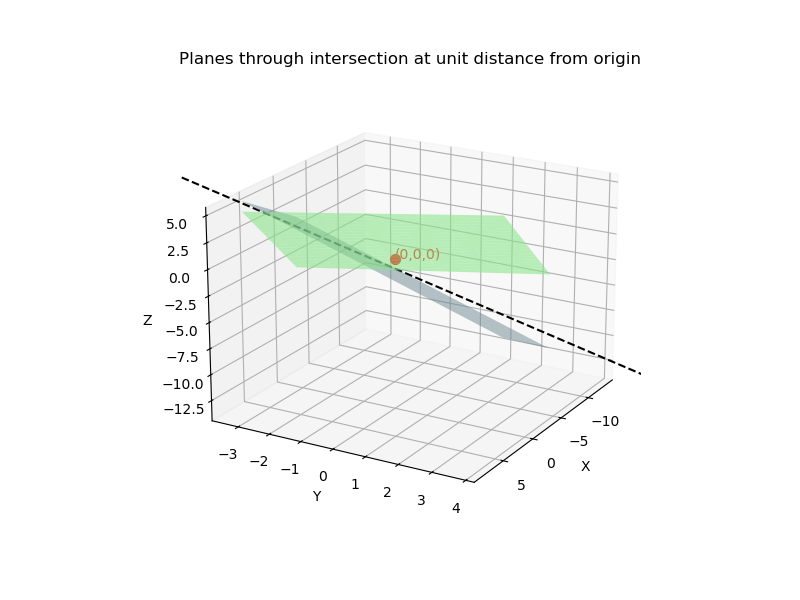
\includegraphics[width=0.75\linewidth]{figs/Figure_1.png}
    \caption{}
    \label{fig:placeholder}
\end{figure}
    
\end{frame}
\end{document}